%\documentclass[
  bibliography=totoc,     % Literatur im Inhaltsverzeichnis
  captions=tableheading,  % Tabellenüberschriften
  titlepage=firstiscover, % Titelseite ist Deckblatt
]{scrartcl}

% Paket float verbessern
\usepackage{scrhack}

% Warnung, falls nochmal kompiliert werden muss
\usepackage[aux]{rerunfilecheck}

% unverzichtbare Mathe-Befehle
\usepackage{amsmath}
% viele Mathe-Symbole
\usepackage{amssymb}
% Erweiterungen für amsmath
\usepackage{mathtools}

% Fonteinstellungen
\usepackage{fontspec}
% Latin Modern Fonts werden automatisch geladen
% Alternativ zum Beispiel:
%\setromanfont{Libertinus Serif}
%\setsansfont{Libertinus Sans}
%\setmonofont{Libertinus Mono}

% Wenn man andere Schriftarten gesetzt hat,
% sollte man das Seiten-Layout neu berechnen lassen
\recalctypearea{}

% deutsche Spracheinstellungen
\usepackage[ngerman]{babel}


\usepackage[
  math-style=ISO,    % ┐
  bold-style=ISO,    % │
  sans-style=italic, % │ ISO-Standard folgen
  nabla=upright,     % │
  partial=upright,   % │
  mathrm=sym,        % ┘
  warnings-off={           % ┐
    mathtools-colon,       % │ unnötige Warnungen ausschalten
    mathtools-overbracket, % │
  },                       % ┘
]{unicode-math}

% traditionelle Fonts für Mathematik
\setmathfont{Latin Modern Math}
% Alternativ zum Beispiel:
%\setmathfont{Libertinus Math}

\setmathfont{XITS Math}[range={scr, bfscr}]
\setmathfont{XITS Math}[range={cal, bfcal}, StylisticSet=1]

% Zahlen und Einheiten
\usepackage[
  locale=DE,                   % deutsche Einstellungen
  separate-uncertainty=true,   % immer Unsicherheit mit \pm
  per-mode=symbol-or-fraction, % / in inline math, fraction in display math
]{siunitx}

% chemische Formeln
\usepackage[
  version=4,
  math-greek=default, % ┐ mit unicode-math zusammenarbeiten
  text-greek=default, % ┘
]{mhchem}

% richtige Anführungszeichen
\usepackage[autostyle]{csquotes}

% schöne Brüche im Text
\usepackage{xfrac}

% Standardplatzierung für Floats einstellen
\usepackage{float}
\floatplacement{figure}{htbp}
\floatplacement{table}{htbp}

% Floats innerhalb einer Section halten
\usepackage[
  section, % Floats innerhalb der Section halten
  below,   % unterhalb der Section aber auf der selben Seite ist ok
]{placeins}

% Seite drehen für breite Tabellen: landscape Umgebung
\usepackage{pdflscape}

% Captions schöner machen.
\usepackage[
  labelfont=bf,        % Tabelle x: Abbildung y: ist jetzt fett
  font=small,          % Schrift etwas kleiner als Dokument
  width=0.9\textwidth, % maximale Breite einer Caption schmaler
]{caption}
% subfigure, subtable, subref
\usepackage{subcaption}

% Grafiken können eingebunden werden
\usepackage{graphicx}

% schöne Tabellen
\usepackage{tabularray}
\UseTblrLibrary{booktabs, siunitx}

% Verbesserungen am Schriftbild
\usepackage{microtype}

% Literaturverzeichnis
\usepackage[
  backend=biber,
]{biblatex}
% Quellendatenbank
\addbibresource{lit.bib}
\addbibresource{programme.bib}

% Hyperlinks im Dokument
\usepackage[
  german,
  unicode,        % Unicode in PDF-Attributen erlauben
  pdfusetitle,    % Titel, Autoren und Datum als PDF-Attribute
  pdfcreator={},  % ┐ PDF-Attribute säubern
  pdfproducer={}, % ┘
]{hyperref}
% erweiterte Bookmarks im PDF
\usepackage{bookmark}

% Trennung von Wörtern mit Strichen
\usepackage[shortcuts]{extdash}

\author{%
  Vincent Wirsdörfer\\%
  \href{mailto:vincent.wirsdoerfer@udo.edu}{authorA@udo.edu}%
  \and%
  Joris Daus\\%
  \href{mailto:joris.daus@udo.edu}{authorB@udo.edu}%
}
\publishers{TU Dortmund – Fakultät Physik}


%\begin{document}
\section{Auswertung}
\label{sec:Auswertung}

Aus dem Experiment lassen sich die Schallgeschwindigkeiten in Acryl und Aluminium herleiten. Außerdem kann die 
Dämpfung in Acryl für die jeweiligen Ultraschallköpfe bestimmt werden. Es wird außerdem eine Kalibrierkurve für 
die Erkennung des Füllstandes aufgenommen.
Zuerst wird jedoch ein Einblick in das Programm gewährt. Zur Wellenlängenbestimmung soll mehrfach die Periodendauer 
bestimmt werden. Dies geschieht, indem mit dem Computerprogramm die Perdiodendauer an den markierten Stellen 
ausgewertet wird. So wird fünf mal ein Wert von $t = \qty{5e-7}{\second}$ gemessen. Wird dies nun mit dem 
Literaturwert von Acryl für die Schallgeschwindigkeit von \qty{2730}{\meter \per \second} multipliziert, so erhält 
man eine Wellenlänge von $\lambda = \qty{1.831e-10}{\meter}$. Dies ist die Wellenlänge des Schalls in Acryl. Die entsprechende 
Frequenz ist der Kehrwert der Perdiodendauer und somit $f=\qty{2}{\mega\hertz}$, was genau der Frequenz der 
Ultraschallsonde entspricht.
\begin{figure}
    \centering
    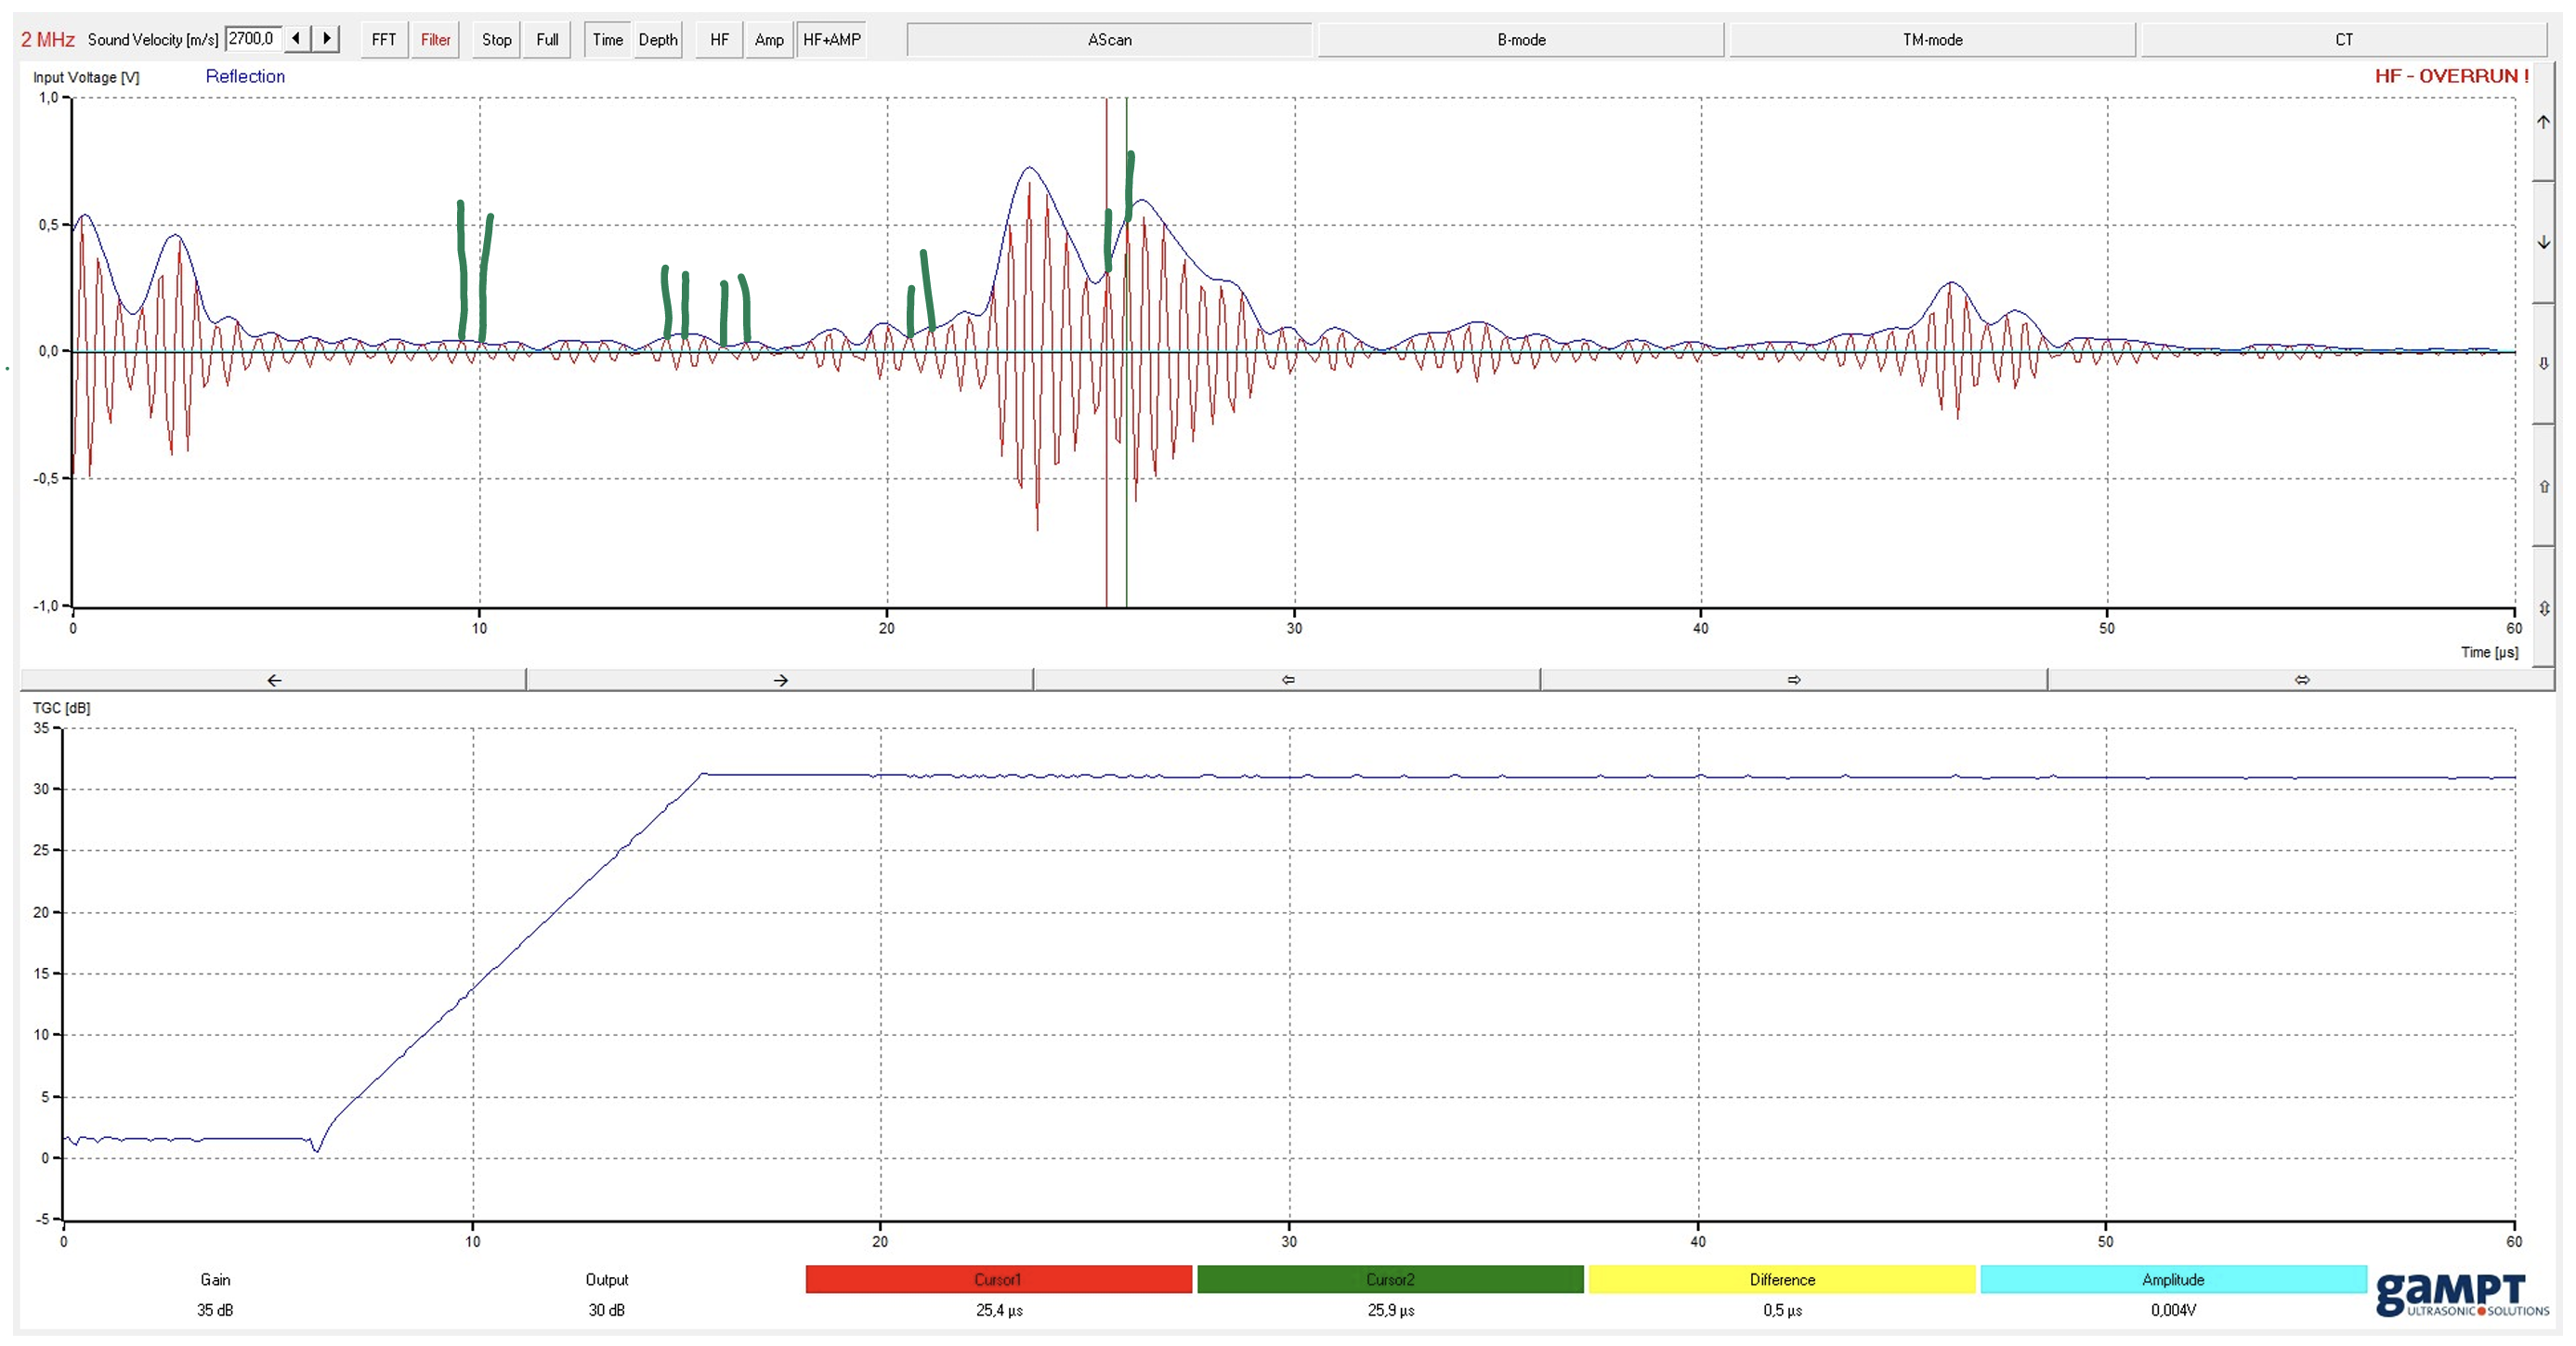
\includegraphics[width=0.9\textwidth]{PC.png}
\end{figure}

\subsection{Schallgeschwindigkeiten}
Zu Beginn werden die Schallgeschwindigkeiten in Acryl und Aluminium bestimmt. Die gemessenen Zeitdifferenzen 
werden nun gegen die zweifache Höhe der Zylinder aufgetragen. Es wird die zweifache Höhe genommen, da dies die 
Wegdifferenz ist, welcher der Schall zurücklegt. Die aufgetragenen Messdaten werden anschließend mittels einer 
Ausgleichsgerade gefittet. Die Steigung dieser Gerade ist nun die Schallgeschwindigkeit.\\

\noindent Dieses Verfahren wird zunächst für Aluminium durchgeführt. So entsteht die folgende Auftragung.

\begin{figure}[H]
    \centering
    \includegraphics[width=0.9\textwidth]{../build/Schall_Alu.pdf}
    \caption{Laufzeit des Schalls gegen zweifache Höhe der Aluminiumzylinder.}
\end{figure}

\noindent Die Steigung der Ausgleichsgerade ergibt eine Schallgeschwindigkeit in Aluminium $v_\text{Alu}$ von 

\begin{align*}
    v_\text{Alu} &= \qty{6.46\pm0.08e3}{\meter \per \second}.
\end{align*}

\noindent Dieses Vorgehen wird nun für die Acrylzylinder wiederholt. So ergibt sich die folgende Auftragung.

\begin{figure}[H]
    \centering
    \includegraphics[width=0.9\textwidth]{../build/Schall_Acryl.pdf}
    \caption{Laufzeit des Schalls gegen zweifache Höhe der Acrylzylinder.}
\end{figure}

\noindent Die Steigung der Ausgleichsgerade ergibt nun eine Schallgeschwindigkeit in Acryl $v_\text{Acryl}$ von 

\begin{align*}
    v_\text{Acryl} &= \qty{2.79\pm0.04e3}{\meter \per \second}.
\end{align*}


\subsection{Dämpfung}
Die Amplitude der Schallwellen in einem Material nehmen mit der Strecke exponentiell ab. Aus diesem Grund 
sollen die Messdaten eingezeichnet und anschließend mit einer e-Funktion der Form $a \symup{e} ^{-bx} +c$ 
gefittet werden. Auf die y-Achse wird der Quotient aus Eingangsspannung $U_0$ und Ausgangsspannung $U$, 
also $\frac{U}{U_0}$ aufgetragen. Auf die x-Achse wird wie bei der Schallgeschwindigkeit die zweifache Höhe 
des Zylinders aufgetragen. 
Dieser gibt an, wie viel Prozent der Eingangsspannung es wieder zurück zum Detektor schaffen. So sind dies 
Relativwerte und nicht mit der Messapparatur in direkter Korrelation. Systematische Fehler sollen so vermieden 
werden. Dieser Teil des Experimentes wird nur für die Acrylzylinder durchgeführt, da für die Aluminiumzylinder 
keine plausiblen Daten aufgenommen werden konnten. \\
\noindent Zu Beginn werden die Daten des \qty{2}{\mega \hertz} Ultraschallkopfes ausgewertet. Die Auftragung 
und der fit mittels \emph{curve\_fit} ergeben den folgenden Plot.

\begin{figure}[H]
    \centering
    \includegraphics[width=0.9\textwidth]{../build/Dämpfungskurve2MHz.pdf}
    \caption{Dämpfung des Schalls in Acryl bei \qty{2}{\mega\hertz}.}
    \label{fig:Kurve2MHz}
\end{figure}

\noindent Der \emph{curve\_fit} berechnet folgende Parameter der e-Funktion:

\begin{align*}
    a &= \num{2.46\pm0.29} \\
    b &= \qty{7.92\pm4.62}{\per \meter} \\
    c &= \num{0.39\pm0.48} \\
\end{align*}

\noindent So ist der Dämpfungsfaktor $\alpha$ auf 

\begin{align*}
    \alpha = b = \qty{8\pm5}{\per \meter}
\end{align*}

\noindent bestimmt.\\

\noindent Die Messung der Acrylzylinder mit dem \qty{2}{\mega\hertz} Ultraschallkopf stellt sich als weniger brauchbar heraus. 
Es wird dennoch versucht eine Dämpfung zu bestimmen. Die Methode eine e-Funktion an die Messdaten anzufügen stellt 
sich als nicht machbar heraus. Der \emph{curve\_fit} kann keine Parameter finden. Auch geeignete Werte vorzugeben 
führt zu keinem Ergebnis. Daher muss eine andere Auswertungsmethode angewandt werden: Die Daten werden logarithmiert, 
um anschließend eine Ausgleichsgerade zu legen. Dazu muss die Funktion zunächst ein wenig umgeschrieben werde. 
Da bei unendlich hohen Zylindern kein Schall reflektiert werden kann, kann die Annahme getroffen werden, dass für 
unendlich hohe Zylinder $\frac{U}{U_0}$ gegen $0$ konvergiert. Daher muss $c=0$ gelten.
So wird die Gleichung 

\begin{equation*}
    \frac{U}{U_0} = a \symup{e} ^{-bx} +c
\end{equation*}

\noindent durch die Annahme vereinfacht  zu

\begin{equation*}
    \frac{U}{U_0} = a \symup{e} ^{-bx}.
\end{equation*}

\noindent Es kann nun der logarithmus gezogen werden, was zu 

\begin{equation*}
    \ln{\frac{U}{U_0}} = {-bx} + \ln{a}
\end{equation*}

\noindent resultiert.

\noindent Der Dämpfungsfaktor ist jetzt die negative Steigung der Ausgleichsgerade. Der Vorfaktor $a$ wird 
zu $\ln{a}$. Es wird nun eine Ausgleichsgerade durch die Daten gezogen. Dies sieht alles zusammen nun folgendermaßen aus

\begin{figure}[H]
    \centering
    \includegraphics[width=0.9\textwidth]{../build/logarithmisch.pdf}
    \caption{Dämpfung des Schalls in Acryl bei \qty{1}{\mega\hertz}.}
\end{figure}

\noindent Diese Ausgleichsgerade besitzt die folgenden Parameter mit der Dämpfung $b$:

\begin{align*}
    -b &= \qty{31.19\pm7.15}{\per \meter} \\
    \ln{a} &= \num{0.89\pm0.84} \\
\end{align*}

\noindent Plottet man nun die Kurve mit den über die lineare Ausgleichsgerade berechneten Parametern und wählt das $c$ entsprechend, 
so entsteht die folgende Auftragung.

\begin{figure}[H]
    \centering
    \includegraphics[width=0.9\textwidth]{../build/Dämpfungskurve1MHz.pdf}
    \caption{Dämpfung des Schalls in Acryl bei \qty{1}{\mega\hertz}.}
\end{figure}



\subsection{Kalibrierkurve}
Die Ultraschalltechnik kann auch zur Bestimmung der Füllhöhen von Gefäßen eingesetzt werden. Dazu wird für das jeweilige Gefäß 
eine Kalibrierkurve aufgenommen. Diese Kalibrierkurve soll nun ermittelt werden. \\
\noindent Die Laufzeit wird als Funktion des Füllstandes des Erlenmeyerkolbens aufgetragen. Da der Erlenmeyerkolben 
die Geometrische Form eines Kegels hat, nimmt die Füllhöhe quadratisch mit dem Volumen zu. Aus diesem Grund werden die Daten 
mit einem Polynom zweiten Grades der Form $ax^2 +bx +c$ gefittet. So entsteht der folgende Graphik.

\begin{figure}[H]
    \centering
    \includegraphics[width=0.9\textwidth]{../build/Kalibrierkurve.pdf}
    \caption{Kalibrierkurve eines Erlenmeyerkolbens.}
    \label{fig:Kalibrierkurve}
\end{figure}

\noindent Die ermittelte Kalibrierkurve besitzt so die folgende Form

\begin{equation*}
    f(x)= \qty{6.073\pm0.479e-4}{\micro \second \per \milli \liter \squared } \cdot x^2   +  
          \qty{0.107\pm0.012}{\micro \second \per \milli \liter}              \cdot x     +
          \qty{10.71\pm0.698}{\micro \second }
\end{equation*}


%\end{document}
